Loading initial resources:

\begin{Shaded}
\begin{Highlighting}[]
\KeywordTok{library}\NormalTok{(tidyverse)}
\KeywordTok{library}\NormalTok{(magrittr)}
\KeywordTok{library}\NormalTok{(geneplast)}
\KeywordTok{library}\NormalTok{(ape)}
\KeywordTok{library}\NormalTok{(XML)}
\KeywordTok{library}\NormalTok{(rentrez)}
\KeywordTok{library}\NormalTok{(neurotransmissionevolution)}

\KeywordTok{data}\NormalTok{(}
\NormalTok{  cogs,}
\NormalTok{  gene_cogs,}
\NormalTok{  string_eukaryotes,}
  \DataTypeTok{package =} \StringTok{"neurotransmissionevolution"}
\NormalTok{)}

\NormalTok{phyloTree <-}\StringTok{ }\KeywordTok{read.tree}\NormalTok{(}\StringTok{"../data/hybrid_tree_modified.nwk"}\NormalTok{) }\OperatorTok\StringTok{ }\KeywordTok{rotatePhyloTree}\NormalTok{(}\StringTok{"9606"}\NormalTok{)}
\end{Highlighting}
\end{Shaded}

We perform some minor data formatting before feeding it to geneplast

\begin{Shaded}
\begin{Highlighting}[]
\CommentTok{# Formating cogdata column names for geneplast}
\NormalTok{cogs }\OperatorTok\StringTok{ }\KeywordTok{select}\NormalTok{(}\DataTypeTok{protein_id =}\NormalTok{ string_id, }\DataTypeTok{ssp_id =}\NormalTok{ taxid, cog_id)}

\CommentTok{# Adding species names to taxid tree}
\NormalTok{phyloTree }\OperatorTok\StringTok{ }\KeywordTok{list_modify}\NormalTok{(}
  \DataTypeTok{tip.alias =}\NormalTok{ string_eukaryotes }\OperatorTok\StringTok{ }\NormalTok{string_name[}\KeywordTok{match}\NormalTok{(phyloTree[[}\StringTok{"tip.label"}\NormalTok{]], taxid)]}
\NormalTok{)}
\end{Highlighting}
\end{Shaded}

\hypertarget{geneplast}{%
\subsubsection{Geneplast}\label{geneplast}}

Geneplast's \texttt{groot.preprocess} function structures an
\texttt{ogr} object on which \texttt{groot} will perform the rooting. We
then retrieve the numeric root (\texttt{groot.get("results")}) for the
\texttt{cogs\_of\_interest}, that is, orthologous groups pertaining to
neurotransmission genes.

\begin{Shaded}
\begin{Highlighting}[]
\NormalTok{cogs_of_interest <-}\StringTok{ }\NormalTok{gene_cogs }\OperatorTok\StringTok{ }\KeywordTok{pull}\NormalTok{(cog_id) }\OperatorTok\StringTok{ }\NormalTok{unique}

\NormalTok{ogr <-}\StringTok{ }\KeywordTok{groot.preprocess}\NormalTok{(}
  \DataTypeTok{cogdata   =}\NormalTok{ cogs,}
  \DataTypeTok{phyloTree =}\NormalTok{ phyloTree,}
  \DataTypeTok{spid      =} \StringTok{"9606"}\NormalTok{,}
  \DataTypeTok{cogids    =}\NormalTok{ cogs_of_interest}
\NormalTok{)}

\NormalTok{roots <-}\StringTok{ }\KeywordTok{groot}\NormalTok{(ogr, }\DataTypeTok{nPermutations =} \DecValTok{1}\NormalTok{) }\OperatorTok
\StringTok{  }\KeywordTok{groot.get}\NormalTok{(}\StringTok{"results"}\NormalTok{) }\OperatorTok
\StringTok{  }\KeywordTok{rownames_to_column}\NormalTok{(}\StringTok{"cog_id"}\NormalTok{) }\OperatorTok
\StringTok{  }\KeywordTok{select}\NormalTok{(cog_id, }\DataTypeTok{root =}\NormalTok{ Root) }\OperatorTok
\StringTok{  }\KeywordTok{write_tsv}\NormalTok{(}\StringTok{"geneplast_roots.tsv"}\NormalTok{)}
\end{Highlighting}
\end{Shaded}

\hypertarget{clade-names}{%
\subsubsection{Clade names}\label{clade-names}}

Each root branches to a clade that diverged from humans some time in the
past. It is nice to have these clades taxonomically named to ease our
interpretation. Unlike NCBI Taxonomy, TimeTree's internal nodes are not
named. Therefore, we query the NCBI Taxonomy API to try to find most
clade names automatically. It is important to note that we are using a
hybrid tree primarily built from TimeTree data. This means NCBI Taxonomy
naming will not perfectly match clades in our tree. For instance, root
\#36 branches to a clade containing 38 species from the SAR supergroup,
but also 1 species from the Haptista rank, namely \emph{Emiliania
huxleyi}. The Haptista group is a sister clade to SAR, so it might be
the case that \emph{Emiliania huxleyi} is actually correctly placed
together with SAR species by TimeTree, given their evolutionary
proximity. Resolving these naming conflicts is not trivial and falls out
of our scope.

\begin{Shaded}
\begin{Highlighting}[]
\CommentTok{# Querying NCBI Taxonomy with our taxids}
\NormalTok{lineages <-}\StringTok{ }\KeywordTok{entrez_fetch}\NormalTok{(}
  \DataTypeTok{db      =} \StringTok{"taxonomy"}\NormalTok{,}
  \DataTypeTok{id      =}\NormalTok{ string_eukaryotes[[}\StringTok{"new_taxid"}\NormalTok{]],}
  \DataTypeTok{rettype =} \StringTok{"xml"}\NormalTok{,}
  \DataTypeTok{retmode =} \StringTok{"xml"}\NormalTok{,}
  \DataTypeTok{parsed  =} \OtherTok{TRUE}
\NormalTok{)}

\CommentTok{# Parsing the XML result and retrieving lineage data}
\NormalTok{string_eukaryotes }\OperatorTok\StringTok{ }\KeywordTok{mutate}\NormalTok{(}
  \DataTypeTok{root        =}\NormalTok{ ogr}\OperatorTok{@}\NormalTok{tree}\OperatorTok{$}\NormalTok{tip.group[taxid],}
  \DataTypeTok{lineage_txt =} \KeywordTok{xpathSApply}\NormalTok{(lineages, }\StringTok{"//Lineage"}\NormalTok{, XML}\OperatorTok{::}\NormalTok{xmlValue)}
\NormalTok{)}

\CommentTok{# Writing all lineage data to manually check for edge cases}
\NormalTok{string_eukaryotes }\OperatorTok
\StringTok{  }\KeywordTok{select}\NormalTok{(root, lineage_txt) }\OperatorTok
\StringTok{  }\KeywordTok{arrange}\NormalTok{(root, lineage_txt) }\OperatorTok
\StringTok{  }\KeywordTok{write_tsv}\NormalTok{(}\StringTok{"temp/species_lineage.txt"}\NormalTok{)}

\CommentTok{# The following chain of dplyr verbs}
\CommentTok{# is responsible for figuring out the best clade names}
\NormalTok{root_names <-}\StringTok{ }\NormalTok{string_eukaryotes }\OperatorTok
\StringTok{  }
\StringTok{  }\CommentTok{# Long format lineages}
\StringTok{  }\KeywordTok{mutate}\NormalTok{(}
     \DataTypeTok{lineage_split =} \KeywordTok{strsplit}\NormalTok{(lineage_txt, }\StringTok{"; "}\NormalTok{)}
\NormalTok{  ) }\OperatorTok
\StringTok{  }\KeywordTok{unnest_longer}\NormalTok{(}
     \DataTypeTok{col        =}\NormalTok{ lineage_split}
\NormalTok{    ,}\DataTypeTok{values_to  =} \StringTok{"clade_name"}
\NormalTok{    ,}\DataTypeTok{indices_to =} \StringTok{"clade_depth"}
\NormalTok{  ) }\OperatorTok
\StringTok{  }
\StringTok{  }\CommentTok{# Counting and dropping the last group}
\StringTok{  }\KeywordTok{group_by}\NormalTok{(root, clade_depth, clade_name) }\OperatorTok
\StringTok{  }\KeywordTok{tally}\NormalTok{(}\DataTypeTok{sort =} \OtherTok{TRUE}\NormalTok{) }\OperatorTok
\StringTok{  }
\StringTok{  }\CommentTok{# Collapsing lineages by clade depths}
\StringTok{  }\KeywordTok{summarise}\NormalTok{(}
     \DataTypeTok{diverging_rank =} \KeywordTok{n_distinct}\NormalTok{(clade_name) }\OperatorTok{>}\StringTok{ }\DecValTok{1}
\NormalTok{    ,}\DataTypeTok{clade_name     =} \KeywordTok{ifelse}\NormalTok{(diverging_rank, }\KeywordTok{paste0}\NormalTok{(clade_name, }\StringTok{" ("}\NormalTok{, n,}\StringTok{")"}\NormalTok{, }\DataTypeTok{collapse =} \StringTok{"; "}\NormalTok{), clade_name)}
\NormalTok{  ) }\OperatorTok
\StringTok{  }
\StringTok{  }\CommentTok{# Removing diverging ranks after the first one}
\StringTok{  }\KeywordTok{filter}\NormalTok{(}\KeywordTok{cumsum}\NormalTok{(diverging_rank) }\OperatorTok{<=}\StringTok{ }\DecValTok{1}\NormalTok{) }\OperatorTok
\StringTok{  }
\StringTok{  }\CommentTok{# Removing irrelevant basal ranks (eg Eukaryota)}
\StringTok{  }\KeywordTok{group_by}\NormalTok{(clade_depth) }\OperatorTok
\StringTok{  }\KeywordTok{arrange}\NormalTok{(root) }\OperatorTok
\StringTok{  }\KeywordTok{filter}\NormalTok{(}\OperatorTok{!}\NormalTok{(}\KeywordTok{duplicated}\NormalTok{(clade_name) }\OperatorTok{|}\StringTok{ }\KeywordTok{duplicated}\NormalTok{(clade_name, }\DataTypeTok{fromLast =} \OtherTok{TRUE}\NormalTok{)) }\OperatorTok{|}\StringTok{ }\NormalTok{diverging_rank) }\OperatorTok
\StringTok{  }
\StringTok{  }\CommentTok{# Choosing name}
\StringTok{  }\KeywordTok{group_by}\NormalTok{(root) }\OperatorTok
\StringTok{  }\KeywordTok{summarise}\NormalTok{(}\DataTypeTok{clade_name =} \KeywordTok{first}\NormalTok{(clade_name, }\DataTypeTok{order_by =}\NormalTok{ clade_depth)) }\OperatorTok
\StringTok{  }\KeywordTok{write_tsv}\NormalTok{(}\StringTok{"temp/temp_geneplast_clade_names.tsv"}\NormalTok{)}
\end{Highlighting}
\end{Shaded}

Some automatically named clades are resolved by hand. The following
table shows clade names before and after manual checking:

\begin{Shaded}
\begin{Highlighting}[]
\CommentTok{# Loading manually resolved names, based on temp/temp_geneplast_clade_names.tsv}
\NormalTok{lca_names <-}\StringTok{ }\KeywordTok{read_tsv}\NormalTok{(}\StringTok{"geneplast_clade_names.tsv"}\NormalTok{)}

\NormalTok{root_names }\OperatorTok
\StringTok{  }\KeywordTok{rename}\NormalTok{(}\StringTok{"Automatic name"}\NormalTok{ =}\StringTok{ }\NormalTok{clade_name) }\OperatorTok
\StringTok{  }\KeywordTok{inner_join}\NormalTok{(lca_names) }\OperatorTok
\StringTok{  }\KeywordTok{rename}\NormalTok{(}\StringTok{"Corrected name"}\NormalTok{ =}\StringTok{ }\NormalTok{clade_name, }\StringTok{"Root"}\NormalTok{ =}\StringTok{ }\NormalTok{root) }\OperatorTok
\StringTok{  }\NormalTok{knitr}\OperatorTok{::}\KeywordTok{kable}\NormalTok{(}\DataTypeTok{caption =} \StringTok{"Clade names before and after manual checking."}\NormalTok{, }\DataTypeTok{booktabs =} \OtherTok{TRUE}\NormalTok{, }\DataTypeTok{linesep =} \StringTok{""}\NormalTok{) }\OperatorTok
\StringTok{  }\NormalTok{kableExtra}\OperatorTok{::}\KeywordTok{kable_styling}\NormalTok{(}\DataTypeTok{position =} \StringTok{"left"}\NormalTok{, }\DataTypeTok{latex_options =} \KeywordTok{c}\NormalTok{(}\StringTok{"striped"}\NormalTok{, }\StringTok{"HOLD_position"}\NormalTok{))}
\end{Highlighting}
\end{Shaded}

\begin{table}[H]

\caption{\label{tab:unnamed-chunk-6}Clade names before and after manual checking.}
\begin{tabular}[t]{rll}
\toprule
Root & Automatic name & Corrected name\\
\midrule
\rowcolor{gray!6}  1 & Homo & Homo\\
2 & Pan & Pan\\
\rowcolor{gray!6}  3 & Gorilla & Gorilla\\
4 & Ponginae & Ponginae\\
\rowcolor{gray!6}  5 & Hylobatidae & Hylobatidae\\
6 & Cercopithecoidea & Cercopithecoidea\\
\rowcolor{gray!6}  7 & Platyrrhini & Platyrrhini\\
8 & Tarsiiformes & Tarsiiformes\\
\rowcolor{gray!6}  9 & Strepsirrhini & Strepsirrhini\\
10 & Dermoptera & Dermoptera\\
\rowcolor{gray!6}  11 & Scandentia & Scandentia\\
12 & Glires & Glires\\
\rowcolor{gray!6}  13 & Laurasiatheria & Laurasiatheria\\
14 & Afrotheria (6); Xenarthra (1) & Afrotheria\\
\rowcolor{gray!6}  15 & Metatheria & Metatheria\\
16 & Prototheria & Prototheria\\
\rowcolor{gray!6}  17 & Sauropsida & Sauropsida\\
18 & Amphibia & Amphibia\\
\rowcolor{gray!6}  19 & Coelacanthimorpha & Coelacanthimorpha\\
20 & Actinopterygii & Actinopterygii\\
\rowcolor{gray!6}  21 & Tunicata & Tunicata\\
22 & Cephalochordata & Cephalochordata\\
\rowcolor{gray!6}  23 & Echinodermata (1); Hemichordata (1) & Ambulacraria\\
24 & Ecdysozoa (43); Spiralia (2) & Ecdysozoa\\
\rowcolor{gray!6}  25 & Spiralia & Spiralia\\
26 & Cnidaria & Cnidaria\\
\rowcolor{gray!6}  27 & Placozoa & Placozoa\\
28 & Porifera & Porifera\\
\rowcolor{gray!6}  29 & Ctenophora & Ctenophora\\
30 & Opisthokonta (5); Apusozoa (1); Cryptophyceae (1) & Unicellular holozoans\\
\rowcolor{gray!6}  31 & Fungi & Fungi\\
32 & Amoebozoa & Amoebozoa\\
\rowcolor{gray!6}  33 & Viridiplantae & Viridiplantae\\
34 & Discoba (6); Metamonada (1); Sar (1) & Discoba\\
\rowcolor{gray!6}  35 & Rhodophyta & Rhodophyta\\
36 & Sar (38); Haptista (1) & SAR\\
\rowcolor{gray!6}  37 & Metamonada & Metamonada\\
\bottomrule
\end{tabular}
\end{table}

\hypertarget{phyletic-patterns}{%
\subsubsection{Phyletic patterns}\label{phyletic-patterns}}

Visualizing the presence/absence matrix according to inferred roots and
species' clades

\begin{Shaded}
\begin{Highlighting}[]
\NormalTok{lca_names }\OperatorTok\StringTok{ }\KeywordTok{rename}\NormalTok{(}\StringTok{"lca"}\NormalTok{ =}\StringTok{ }\NormalTok{root)}

\NormalTok{lca_spp <-}\StringTok{ }\NormalTok{ogr}\OperatorTok{@}\NormalTok{spbranches }\OperatorTok
\StringTok{  }\KeywordTok{rename}\NormalTok{(}\StringTok{"taxid"}\NormalTok{ =}\StringTok{ }\NormalTok{ssp_id, }\StringTok{"species"}\NormalTok{ =}\StringTok{ }\NormalTok{ssp_name, }\StringTok{"lca"}\NormalTok{ =}\StringTok{ `}\DataTypeTok{9606}\StringTok{`}\NormalTok{) }\OperatorTok
\StringTok{  }\KeywordTok{mutate}\NormalTok{(}\DataTypeTok{taxid_order =} \KeywordTok{row_number}\NormalTok{())}
  
\CommentTok{# Saving for use in abundance computation}
\NormalTok{lca_spp }\OperatorTok\StringTok{ }\KeywordTok{select}\NormalTok{(lca, taxid, taxid_order) }\OperatorTok\StringTok{ }\KeywordTok{write_tsv}\NormalTok{(}\StringTok{"geneplast_clade_taxids.tsv"}\NormalTok{)}

\NormalTok{cog_pam <-}\StringTok{ }\NormalTok{ogr}\OperatorTok{@}\NormalTok{orthoct[,}\OperatorTok{-}\DecValTok{1}\NormalTok{]}

\NormalTok{long_pam <-}\StringTok{ }\NormalTok{cog_pam }\OperatorTok
\StringTok{  }\KeywordTok{rownames_to_column}\NormalTok{(}\StringTok{"taxid"}\NormalTok{) }\OperatorTok
\StringTok{  }\KeywordTok{pivot_longer}\NormalTok{(}\OperatorTok{-}\NormalTok{taxid, }\DataTypeTok{names_to =} \StringTok{"cog_id"}\NormalTok{) }\OperatorTok
\StringTok{  }\KeywordTok{left_join}\NormalTok{(lca_spp) }\OperatorTok
\StringTok{  }\KeywordTok{left_join}\NormalTok{(lca_names) }\OperatorTok
\StringTok{  }\KeywordTok{left_join}\NormalTok{(roots) }\OperatorTok
\StringTok{  }\KeywordTok{mutate}\NormalTok{(}
    \DataTypeTok{cog_id       =} \KeywordTok{fct_reorder}\NormalTok{(cog_id, root),}
    \DataTypeTok{species      =} \KeywordTok{fct_reorder}\NormalTok{(species, }\KeywordTok{desc}\NormalTok{(taxid_order)),}
    \DataTypeTok{clade_name   =} \KeywordTok{fct_reorder}\NormalTok{(clade_name, lca),}
    \DataTypeTok{root         =} \KeywordTok{as_factor}\NormalTok{(root),}
    \DataTypeTok{clade_stripe =} \KeywordTok{as.numeric}\NormalTok{(}\KeywordTok{as_factor}\NormalTok{(lca)) }\OperatorTok\StringTok{ }\DecValTok{2} \OperatorTok{==}\StringTok{ }\DecValTok{0}
\NormalTok{  ) }\OperatorTok
\StringTok{  }\CommentTok{# Stripe every other species}
\StringTok{  }\KeywordTok{group_by}\NormalTok{(cog_id) }\OperatorTok
\StringTok{  }\KeywordTok{mutate}\NormalTok{(}\DataTypeTok{spp_stripe =} \KeywordTok{as.numeric}\NormalTok{(species) }\OperatorTok\StringTok{ }\DecValTok{2} \OperatorTok{==}\StringTok{ }\DecValTok{0}\NormalTok{) }\OperatorTok
\StringTok{  }\CommentTok{# Removing empty tiles}
\StringTok{  }\KeywordTok{filter}\NormalTok{(value }\OperatorTok{==}\StringTok{ }\DecValTok{1}\NormalTok{) }\OperatorTok
\StringTok{  }\CommentTok{# Stripe every other cog}
\StringTok{  }\KeywordTok{group_by}\NormalTok{(taxid) }\OperatorTok
\StringTok{  }\KeywordTok{mutate}\NormalTok{(}\DataTypeTok{cog_stripe =} \KeywordTok{as.numeric}\NormalTok{(cog_id) }\OperatorTok\StringTok{ }\DecValTok{2} \OperatorTok{==}\StringTok{ }\DecValTok{0}\NormalTok{)}

\KeywordTok{ggplot}\NormalTok{(long_pam, }\KeywordTok{aes}\NormalTok{(}\DataTypeTok{x =}\NormalTok{ cog_id, }\DataTypeTok{y =}\NormalTok{ species)) }\OperatorTok{+}
\StringTok{  }\KeywordTok{geom_tile}\NormalTok{(}\KeywordTok{aes}\NormalTok{(}\DataTypeTok{fill =}\NormalTok{ clade_stripe }\OperatorTok{+}\StringTok{ }\FloatTok{0.3} \OperatorTok{*}\StringTok{ }\KeywordTok{xor}\NormalTok{(spp_stripe, cog_stripe))) }\OperatorTok{+}
\StringTok{  }\KeywordTok{scale_fill_gradient}\NormalTok{(}\DataTypeTok{low =} \StringTok{"#424242"}\NormalTok{, }\DataTypeTok{high =} \StringTok{"#212121"}\NormalTok{) }\OperatorTok{+}
\StringTok{  }\KeywordTok{facet_grid}\NormalTok{(clade_name }\OperatorTok{~}\StringTok{ }\NormalTok{root, }\DataTypeTok{scales =} \StringTok{"free"}\NormalTok{, }\DataTypeTok{space =} \StringTok{"free"}\NormalTok{) }\OperatorTok{+}
\StringTok{  }\KeywordTok{xlab}\NormalTok{(}\StringTok{"COGs"}\NormalTok{) }\OperatorTok{+}
\StringTok{  }\KeywordTok{ylab}\NormalTok{(}\StringTok{"Species"}\NormalTok{) }\OperatorTok{+}
\StringTok{  }\KeywordTok{theme}\NormalTok{(}
     \DataTypeTok{legend.position    =} \StringTok{"none"}
\NormalTok{    ,}\DataTypeTok{strip.background   =} \KeywordTok{element_blank}\NormalTok{()}
\NormalTok{    ,}\DataTypeTok{strip.text.x       =} \KeywordTok{element_text}\NormalTok{(}\DataTypeTok{size =} \DecValTok{4}\NormalTok{, }\DataTypeTok{angle =} \DecValTok{0}\NormalTok{, }\DataTypeTok{vjust =} \DecValTok{0}\NormalTok{)}
\NormalTok{    ,}\DataTypeTok{strip.text.y       =} \KeywordTok{element_text}\NormalTok{(}\DataTypeTok{size =} \DecValTok{5}\NormalTok{, }\DataTypeTok{angle =} \DecValTok{0}\NormalTok{, }\DataTypeTok{hjust =} \DecValTok{0}\NormalTok{)}
\NormalTok{    ,}\DataTypeTok{axis.text.x        =} \KeywordTok{element_text}\NormalTok{(}\DataTypeTok{size =} \DecValTok{3}\NormalTok{, }\DataTypeTok{angle =} \DecValTok{-45}\NormalTok{, }\DataTypeTok{vjust =} \DecValTok{0}\NormalTok{, }\DataTypeTok{hjust =} \FloatTok{0.125}\NormalTok{)}
\NormalTok{    ,}\DataTypeTok{axis.text.y        =} \KeywordTok{element_text}\NormalTok{(}\DataTypeTok{size =} \DecValTok{4}\NormalTok{)}
\NormalTok{    ,}\DataTypeTok{axis.title         =} \KeywordTok{element_text}\NormalTok{(}\DataTypeTok{size =} \DecValTok{8}\NormalTok{)}
\NormalTok{    ,}\DataTypeTok{axis.ticks         =} \KeywordTok{element_line}\NormalTok{(}\DataTypeTok{size =} \FloatTok{0.25}\NormalTok{)}
\NormalTok{    ,}\DataTypeTok{panel.grid.major.y =} \KeywordTok{element_line}\NormalTok{(}\DataTypeTok{size =} \FloatTok{0.25}\NormalTok{)}
\NormalTok{    ,}\DataTypeTok{panel.grid.major.x =} \KeywordTok{element_blank}\NormalTok{()}
\NormalTok{    ,}\DataTypeTok{panel.spacing      =} \KeywordTok{unit}\NormalTok{(}\FloatTok{0.25}\NormalTok{, }\StringTok{"pt"}\NormalTok{)}
\NormalTok{    ,}\DataTypeTok{plot.margin        =} \KeywordTok{unit}\NormalTok{(}\KeywordTok{c}\NormalTok{(}\DecValTok{0}\NormalTok{,}\DecValTok{0}\NormalTok{,}\DecValTok{0}\NormalTok{,}\DecValTok{0}\NormalTok{), }\StringTok{"mm"}\NormalTok{)}
\NormalTok{  )}
\end{Highlighting}
\end{Shaded}

\clearpage

\thispagestyle{empty}

\pdfpageheight=33in

\begin{figure}[p]

\caption{Presence of orthologous groups in species. The horizontal axis is grouped according to assigned roots. The vertical axis is grouped by clades. A checkerboard pattern is superimposed to aid visualization.}\label{fig:phyletic_patterns}

{\centering 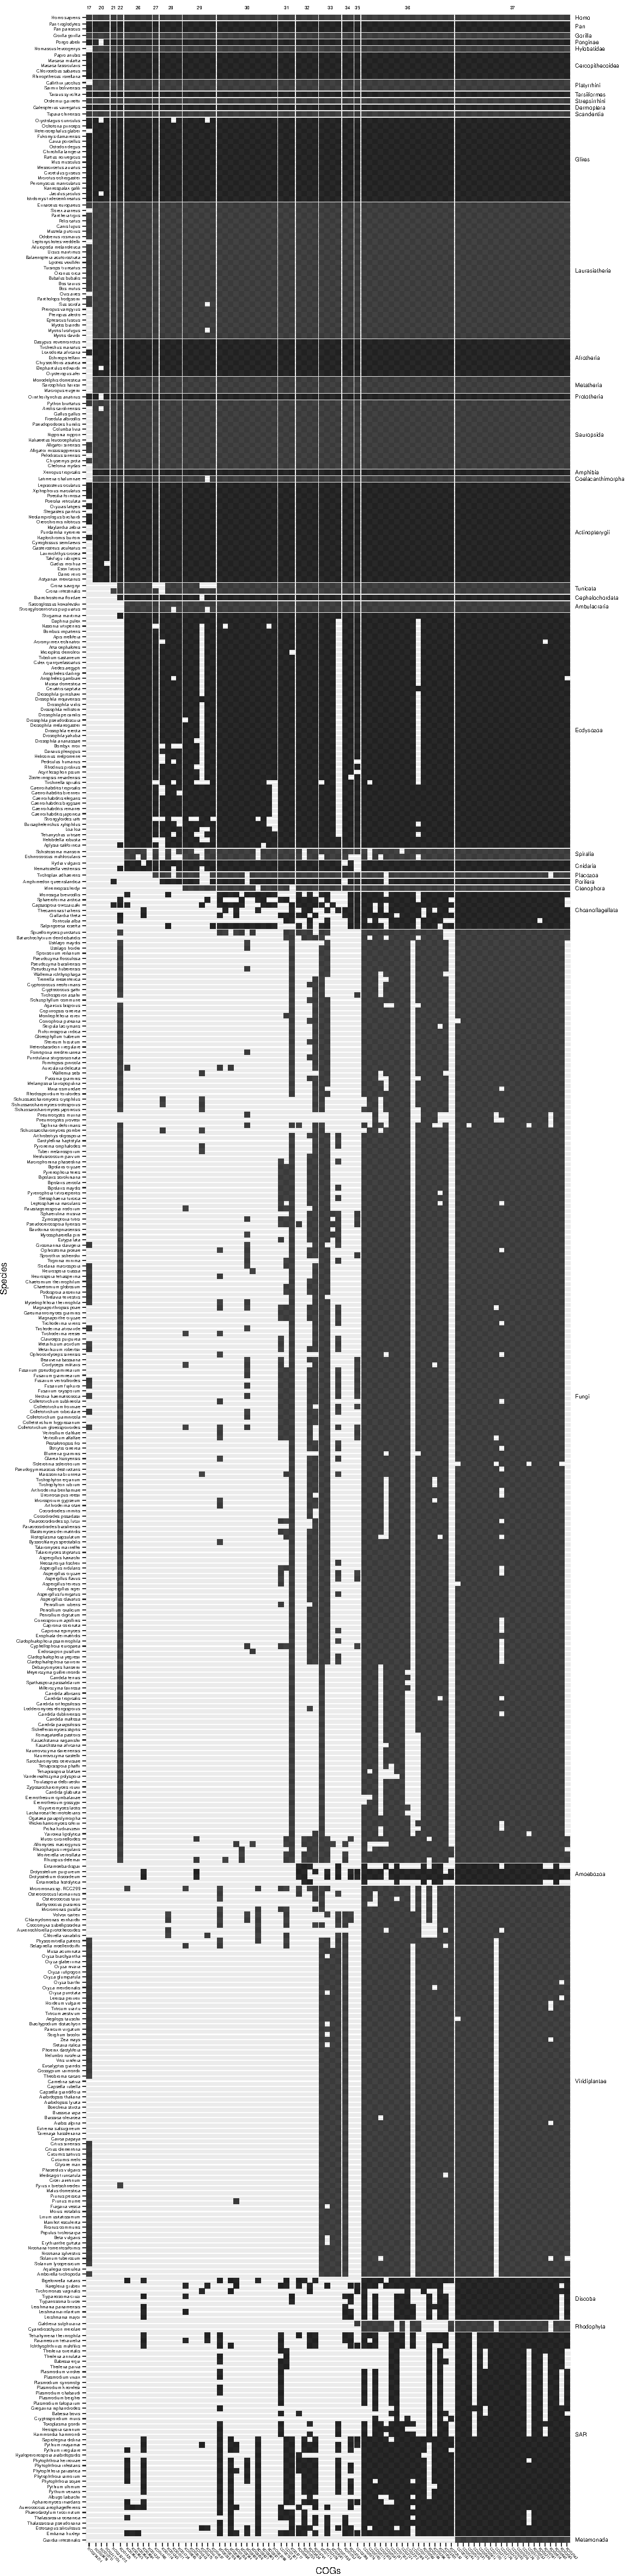
\includegraphics[height=31in, width=7in]{figs/analysis.geneplast.phyletic_patterns-1} }

\end{figure}

\clearpage

\pdfpageheight=11in

\hypertarget{adhesion-genes}{%
\subsubsection{Adhesion genes}\label{adhesion-genes}}

Aditionally\ldots{}

\begin{Shaded}
\begin{Highlighting}[]
\KeywordTok{data}\NormalTok{(}
\NormalTok{  adhesion_genes,}
\NormalTok{  gene_cogs_extra,}
  \DataTypeTok{package =} \StringTok{"neurotransmissionevolution"}
\NormalTok{)}

\NormalTok{cogs_of_interest_extra <-}\StringTok{ }\NormalTok{gene_cogs_extra }\OperatorTok\StringTok{ }\KeywordTok{pull}\NormalTok{(cog_id) }\OperatorTok\StringTok{ }\NormalTok{unique}

\NormalTok{ogr_extra <-}\StringTok{ }\KeywordTok{groot.preprocess}\NormalTok{(}
  \DataTypeTok{cogdata   =}\NormalTok{ cogs,}
  \DataTypeTok{phyloTree =}\NormalTok{ phyloTree,}
  \DataTypeTok{spid      =} \StringTok{"9606"}\NormalTok{,}
  \DataTypeTok{cogids    =}\NormalTok{ cogs_of_interest_extra}
\NormalTok{)}

\NormalTok{roots_extra <-}\StringTok{ }\KeywordTok{groot}\NormalTok{(ogr_extra, }\DataTypeTok{nPermutations =} \DecValTok{1}\NormalTok{) }\OperatorTok
\StringTok{  }\KeywordTok{groot.get}\NormalTok{(}\StringTok{"results"}\NormalTok{) }\OperatorTok
\StringTok{  }\KeywordTok{rownames_to_column}\NormalTok{(}\StringTok{"cog_id"}\NormalTok{) }\OperatorTok
\StringTok{  }\KeywordTok{left_join}\NormalTok{(gene_cogs_extra) }\OperatorTok
\StringTok{  }\KeywordTok{left_join}\NormalTok{(adhesion_genes) }\OperatorTok
\StringTok{  }\KeywordTok{left_join}\NormalTok{(lca_names, }\DataTypeTok{by =} \KeywordTok{c}\NormalTok{(}\StringTok{"Root"}\NormalTok{ =}\StringTok{ "lca"}\NormalTok{))}
\end{Highlighting}
\end{Shaded}

\begin{table}[H]

\caption{\label{tab:unnamed-chunk-8}Adhesion genes in the neural system (KEGG Pathway hsa04514).}
\begin{tabular}[t]{llll}
\toprule
String ID & COG & Symbol & Root\\
\midrule
\rowcolor{gray!6}  ENSP00000329797 & NOG10515 & CADM1 & Human-Actinopterygii LCA (\#20)\\
ENSP00000432943 & NOG16799 & MPZ & Human-Actinopterygii LCA (\#20)\\
\rowcolor{gray!6}  ENSP00000352513 & NOG16799 & MPZL1 & Human-Actinopterygii LCA (\#20)\\
ENSP00000361818 & NOG22019 & SDC4 & Human-Actinopterygii LCA (\#20)\\
\rowcolor{gray!6}  ENSP00000357106 & NOG09962 & CADM3 & Human-Tunicata LCA (\#21)\\
ENSP00000264025 & NOG09962 & NECTIN1 & Human-Tunicata LCA (\#21)\\
\rowcolor{gray!6}  ENSP00000418070 & NOG09962 & NECTIN3 & Human-Tunicata LCA (\#21)\\
ENSP00000370542 & NOG05154 & SDC1 & Human-Ambulacraria LCA (\#23)\\
\rowcolor{gray!6}  ENSP00000307046 & NOG05154 & SDC2 & Human-Ambulacraria LCA (\#23)\\
ENSP00000344468 & NOG05154 & SDC3 & Human-Ambulacraria LCA (\#23)\\
\rowcolor{gray!6}  ENSP00000265077 & NOG02372 & VCAN & Human-Cnidaria LCA (\#26)\\
ENSP00000264638 & KOG3516 & CNTNAP1 & Human-Placozoa LCA (\#27)\\
\rowcolor{gray!6}  ENSP00000354778 & KOG3516 & CNTNAP2 & Human-Placozoa LCA (\#27)\\
ENSP00000359085 & KOG3512 & NTNG1 & Human-Placozoa LCA (\#27)\\
\rowcolor{gray!6}  ENSP00000376921 & KOG3512 & NTNG2 & Human-Placozoa LCA (\#27)\\
ENSP00000447006 & KOG3513 & CNTN1 & Human-Ctenophora LCA (\#29)\\
\rowcolor{gray!6}  ENSP00000330633 & KOG3513 & CNTN2 & Human-Ctenophora LCA (\#29)\\
ENSP00000359077 & KOG3513 & L1CAM & Human-Ctenophora LCA (\#29)\\
\rowcolor{gray!6}  ENSP00000344786 & KOG3513 & NFASC & Human-Ctenophora LCA (\#29)\\
ENSP00000368314 & KOG3513 & NRCAM & Human-Ctenophora LCA (\#29)\\
\rowcolor{gray!6}  ENSP00000261769 & KOG3594 & CDH1 & Human-Unicellular holozoans LCA (\#30)\\
ENSP00000269141 & KOG3594 & CDH2 & Human-Unicellular holozoans LCA (\#30)\\
\rowcolor{gray!6}  ENSP00000379350 & KOG1226 & ITGB1 & Human-Unicellular holozoans LCA (\#30)\\
ENSP00000222573 & KOG1226 & ITGB8 & Human-Unicellular holozoans LCA (\#30)\\
\rowcolor{gray!6}  ENSP00000480132 & KOG3510 & NCAM1 & Human-Unicellular holozoans LCA (\#30)\\
ENSP00000383392 & KOG3510 & NCAM2 & Human-Unicellular holozoans LCA (\#30)\\
\rowcolor{gray!6}  ENSP00000350364 & KOG3510 & NEGR1 & Human-Unicellular holozoans LCA (\#30)\\
ENSP00000385142 & KOG3514 & NRXN1 & Human-Unicellular holozoans LCA (\#30)\\
\rowcolor{gray!6}  ENSP00000265459 & KOG3514 & NRXN2 & Human-Unicellular holozoans LCA (\#30)\\
ENSP00000451648 & KOG3514 & NRXN3 & Human-Unicellular holozoans LCA (\#30)\\
\rowcolor{gray!6}  ENSP00000367316 & KOG3637 & ITGA8 & Human-Amoebozoa LCA (\#32)\\
ENSP00000261023 & KOG3637 & ITGAV & Human-Amoebozoa LCA (\#32)\\
\rowcolor{gray!6}  ENSP00000376048 & KOG4475 & MAG & Human-Discoba LCA (\#34)\\
ENSP00000392500 & COG2272 & NLGN1 & Human-SAR LCA (\#36)\\
\rowcolor{gray!6}  ENSP00000305288 & COG2272 & NLGN2 & Human-SAR LCA (\#36)\\
ENSP00000351591 & COG2272 & NLGN3 & Human-SAR LCA (\#36)\\
\rowcolor{gray!6}  ENSP00000370485 & COG2272 & NLGN4X & Human-SAR LCA (\#36)\\
ENSP00000249363 & COG4886 & LRRC4 & Human-Metamonada LCA (\#37)\\
\rowcolor{gray!6}  ENSP00000471502 & COG4886 & LRRC4B & Human-Metamonada LCA (\#37)\\
ENSP00000278198 & COG4886 & LRRC4C & Human-Metamonada LCA (\#37)\\
\rowcolor{gray!6}  ENSP00000353030 & COG5599 & PTPRF & Human-Metamonada LCA (\#37)\\
ENSP00000463325 & COG5599 & PTPRM & Human-Metamonada LCA (\#37)\\
\bottomrule
\end{tabular}
\end{table}
